\documentclass[11pt,a4paper]{article}

\usepackage[utf8]{inputenc}
\usepackage[T1]{fontenc}
\usepackage[polish]{babel}
\usepackage{lmodern}
\usepackage[margin=2.5cm]{geometry}
\usepackage{amsmath,amssymb}
\usepackage{graphicx}
\usepackage{booktabs}
\usepackage{makecell}
\usepackage{float}
\usepackage{xcolor}
\usepackage{listings}
\usepackage{enumitem}
\usepackage[hidelinks]{hyperref}

\graphicspath{{wykresy/}}
\setlist{itemsep=2pt}

\lstset{
  language=Python,
  basicstyle=\ttfamily\scriptsize,
  keywordstyle=\color{blue!70!black}\bfseries,
  commentstyle=\color{green!40!black}\itshape,
  stringstyle=\color{red!60!black},
  numbers=left,
  numberstyle=\tiny\color{gray},
  breaklines=true,
  frame=single,
  showstringspaces=false,
  inputencoding=utf8,
  extendedchars=true,
  literate=
    {ą}{{\k{a}}}1 {ć}{{\'c}}1 {ę}{{\k{e}}}1 {ł}{{\l{}}}1 {ń}{{\'n}}1
    {ó}{{\'o}}1 {ś}{{\'s}}1 {ź}{{\'z}}1 {ż}{{\.z}}1
    {Ą}{{\k{A}}}1 {Ć}{{\'C}}1 {Ę}{{\k{E}}}1 {Ł}{{\L{}}}1 {Ń}{{\'N}}1
    {Ó}{{\'O}}1 {Ś}{{\'S}}1 {Ź}{{\'Z}}1 {Ż}{{\.Z}}1
}

\title{Identyfikacja Procesów -- Projekt 1\\[0.3em]
  \large Usuwanie zakłóceń impulsowych z nagrań muzycznych}
\author{Grupa II: Karolina Grodź 193203, Kajetan Powała-Mosiński 193054}
\date{}
\begin{document}
\maketitle

%==============================================================================
\section{Cel projektu}

Celem projektu jest napisanie programu w języku MATLAB lub Python, który
usuwa sztucznie dodane zakłócenia impulsowe (tzw.\ trzaski, kliki)
z około 20-sekundowego nagrania muzycznego. Grupie II przydzielono nagranie
zapisane w pliku \texttt{02.wav}. Zgodnie z treścią zadania eliminacja
zakłóceń przebiega następująco:
\begin{enumerate}
  \item Przyjmuje się model autoregresyjny rzędu~${r = 4}$ do lokalnej
        reprezentacji dynamiki sygnału.
  \item Zmiany parametrów $a_i$ ($i = 1, \dots, r$) modelu AR($r$) śledzi
        się na bieżąco algorytmem ważonych najmniejszych kwadratów (EW-LS).
        W każdym kroku algorytmu detektor zakłóceń impulsowych kwestionuje
        te próbki, dla których moduł błędu predykcji przekracza trzykrotność
        lokalnej wartości odchylenia standardowego błędu resztowego.
  \item Próbki zakwestionowane przez detektor rekonstruuje się metodą
        interpolacji liniowej: zakwestionowaną próbkę zastępuje się średnią
        arytmetyczną sąsiednich, poprawnych próbek sygnału.
\end{enumerate}
Przyjmuje się przy tym, że zakłócenia mogą występować w seriach obejmujących
maksymalnie 4 próbki.

%==============================================================================
\section{Dane}

Plik \texttt{02.wav} zawiera jednokanałowy sygnał o częstotliwości
próbkowania $f_s = 22\,050$~Hz, zapisany 16-bitowymi słowami: 468\,587 próbek,
czyli 21,3~s. Na potrzeby obliczeń próbki przeskalowano do przedziału
$[-1, 1)$ (podzielono przez $2^{15}$).

Sygnał muzyczny nie przekracza amplitudy około $0{,}24$. Zakłócenia mają
postać pojedynczych lub kilkupróbkowych szpilek o amplitudzie dochodzącej do
pełnej skali (rys.~\ref{fig:sygnal}, górny wykres). W nagraniu jest 123
próbki o module większym niż $0{,}3$. Można zatem bezpiecznie założyć, że
należą one do zakłóceń.

%==============================================================================
\section{Opis metody}

Metodę oparto na treści zadania oraz na prezentacji \emph{Elimination of
clicks} prof.~Macieja Niedźwieckiego, będącej częścią wykładu z przedmiotu
Identyfikacja Procesów~\cite{wyklad}. W dalszej części sprawozdania
określenie \emph{wykład} odnosi się do tej prezentacji.

\subsection{Model sygnału}
\label{sec:model}

Lokalnie sygnał opisano modelem AR($r$), $r=4$:
\begin{equation}
  y(k) = \sum_{i=1}^{r} a_i(k)\, y(k-i) + e(k)
       = \boldsymbol{\varphi}^{T}(k)\,\boldsymbol{\theta}(k) + e(k),
\end{equation}
gdzie
$\boldsymbol{\theta}(k) = [a_1(k), \dots, a_r(k)]^T$ jest wektorem
(wolnozmiennych) parametrów,
$\boldsymbol{\varphi}(k) = [x(k-1), \dots, x(k-r)]^T$ wektorem regresji,
a $e(k)$ szumem resztowym. Wektor regresji budowany jest z sygnału już
oczyszczonego $x(\cdot)$: próbki wcześniej uznane za zakłócone są w nim
zastąpione wartościami zrekonstruowanymi (sekcja~\ref{sec:rekonstrukcja}).

\subsection{Algorytm EW-LS}
\label{sec:ewls}

Parametry modelu wyznaczano rekurencyjnie, minimalizując ważone
wykładniczo kryterium
$\sum_{j\le k} \lambda^{k-j}\big(y(j)-\boldsymbol{\varphi}^T(j)\boldsymbol{\theta}\big)^2$,
gdzie $0<\lambda<1$ jest współczynnikiem zapominania. Algorytm w każdym
kroku wyznacza:
\begin{align}
  \varepsilon(k) &= y(k) - \boldsymbol{\varphi}^T(k)\,\hat{\boldsymbol{\theta}}(k-1),
     \label{eq:err}\\
  \mathbf{k}(k) &= \frac{\mathbf{P}(k-1)\,\boldsymbol{\varphi}(k)}
                        {\lambda + \boldsymbol{\varphi}^T(k)\,\mathbf{P}(k-1)\,\boldsymbol{\varphi}(k)},\\
  \hat{\boldsymbol{\theta}}(k) &= \hat{\boldsymbol{\theta}}(k-1) + \mathbf{k}(k)\,\varepsilon(k),\\
  \mathbf{P}(k) &= \frac{1}{\lambda}\left[\mathbf{P}(k-1) -
     \frac{\mathbf{P}(k-1)\boldsymbol{\varphi}(k)\boldsymbol{\varphi}^T(k)\mathbf{P}(k-1)}
          {\lambda + \boldsymbol{\varphi}^T(k)\,\mathbf{P}(k-1)\,\boldsymbol{\varphi}(k)}\right],
\end{align}
z warunkami początkowymi $\hat{\boldsymbol{\theta}}(0)=\mathbf{0}$,
$\mathbf{P}(0) = \delta \mathbf{I}$, $\delta = 100$. Efektywna pamięć
estymatora wynosi około $1/(1-\lambda)$ próbek. Na próbkach zakwestionowanych
przez detektor model nie jest aktualizowany.

\paragraph{Zabezpieczenia numeryczne.}
Sygnał audio próbkowany z częstotliwością 22~kHz jest silnie skorelowany,
a macierz kowariancji wektora regresji jest źle uwarunkowana. W takich
warunkach błędy zaokrągleń szybko odbierają macierzy $\mathbf{P}$ symetrię
i dodatnią określoność, co prowadzi do rozbieżności estymat. Dlatego:
\begin{itemize}
  \item macierz $\mathbf{P}$ aktualizowana jest w postaci symetrycznej
        podanej wyżej, a po każdym kroku dodatkowo symetryzowana:
        $\mathbf{P} \leftarrow \tfrac12(\mathbf{P}+\mathbf{P}^T)$,
  \item ślad macierzy jest ograniczony: jeśli
        $\operatorname{tr}\mathbf{P}(k) > 10^4$, to macierz jest
        przeskalowywana do śladu równego $10^4$. Zapobiega to
        niekontrolowanemu wzrostowi $\mathbf{P}$ w słabo pobudzanych
        kierunkach przestrzeni parametrów (\emph{estimator windup}).
\end{itemize}

\subsection{Detektor zakłóceń}
\label{sec:detektor}

Zgodnie z wykładem~\cite{wyklad} lokalną wariancję błędu predykcji
jednokrokowej $\varepsilon(k) = y(k) - \hat y(k\,|\,k-1)$ estymowano jako
średnią z okna przesuwnego obejmującego $M$ poprzednich błędów:
\begin{equation}
  \hat\sigma^2_\varepsilon(k) = \frac{1}{M}\sum_{i=1}^{M} \varepsilon^2(k-i),
  \qquad M = 20 .
\end{equation}
Do okna trafiają wyłącznie błędy próbek uznanych za poprawne. Gdyby
uwzględniać błędy próbek zakłóconych (rzędu $1$), estymata
$\hat\sigma_\varepsilon$ byłaby zawyżona przez kolejne $M$ próbek
i maskowałaby zakłócenia występujące tuż po sobie.

Wynik detektora $\hat d(k)$ wyznaczany jest według reguły decyzyjnej
z wykładu:
\begin{equation}
  \hat d(k) =
  \begin{cases}
    0 & \text{gdy } |\varepsilon(k)| \le \mu\,\hat\sigma_\varepsilon(k), \\
    1 & \text{gdy } |\varepsilon(k)| > \mu\,\hat\sigma_\varepsilon(k),
  \end{cases}
  \qquad \mu = 3 ,
  \label{eq:det}
\end{equation}
gdzie $\hat d(k)=1$ oznacza próbkę zakwestionowaną. Wielkość
$\mu\,\hat\sigma_\varepsilon(k)$ to próg kwalifikujący próbkę jako błędną;
jego przebieg pokazano na rys.~\ref{fig:prog}. Według wykładu
w zastosowaniach audio próg $\mu$ dobiera się empirycznie, zwykle
z przedziału $[3, 5]$. Treść zadania narzuca wartość $\mu = 3$. Detekcja
jest włączana po 500 próbkach, gdy estymaty $\hat{\boldsymbol\theta}$ zdążą
się ustalić.

\subsection{Wyznaczanie długości serii zakłóceń}
\label{sec:seria}

Zakwestionowanie próbki $y(k)$ rozpoczyna potencjalną serię zakłóceń
o długości $m \in \{1,\dots,4\}$. Długość serii wyznaczana jest przez
sprawdzenie kolejnych próbek $y(k+1), \dots, y(k+4)$ względem predykcji
wielokrokowej obliczonej z ostatnich poprawnych próbek
$x(k-1),\dots,x(k-r)$. Predykcję $\hat y(k+j\,|\,k-1)$ uzyskuje się,
stosując rekurencyjnie model AR z parametrami $\hat{\boldsymbol\theta}(k-1)$,
przy czym w miejsce nieznanych próbek $y(k),\dots,y(k+j-1)$ podstawia się
ich predykcje.

Wariancja błędu predykcji $h$-krokowej jest większa niż jednokrokowej:
\begin{equation}
  \sigma_h^2 = \hat\sigma^2_\varepsilon \sum_{i=0}^{h-1} \psi_i^2, \qquad
  \psi_0 = 1,\quad \psi_i = \sum_{j=1}^{\min(i,r)} \hat a_j\, \psi_{i-j},
\end{equation}
gdzie $\psi_i$ jest odpowiedzią impulsową filtru $1/A(z^{-1})$ modelu AR.
Długością serii jest najmniejsze $m$, dla którego próbka $y(k+m)$ jest
zgodna z predykcją:
\begin{equation}
  |y(k+m) - \hat y(k+m\,|\,k-1)| \le \mu\, \sigma_{m+1}.
\end{equation}
Jeśli żadna z próbek $y(k+1),\dots,y(k+4)$ nie spełnia tego warunku,
odchylenie nie jest traktowane jako zakłócenie impulsowe, lecz jako
rzeczywista zmiana charakteru sygnału (np.\ atak dźwięku). Próbka $y(k)$
zostaje wtedy przyjęta jako poprawna i użyta do aktualizacji modelu.

Skalowanie progu przez $\sigma_{m+1}$ jest niezbędne. W cichych fragmentach
nagrania błąd predykcji wielokrokowej dla poprawnych próbek następujących
po trzasku przekracza próg jednokrokowy $3\hat\sigma_\varepsilon$. Bez
skalowania seria wydłużałaby się ponad 4 próbki, a trzask byłby błędnie
przepuszczany.

\subsection{Rekonstrukcja próbek}
\label{sec:rekonstrukcja}

Zakwestionowane próbki zastępowano interpolacją liniową między ostatnią
poprawną próbką $x(k-1)$ a pierwszą poprawną próbką po serii $y(k+m)$:
\begin{equation}
  x(k+i-1) = x(k-1) + \frac{i}{m+1}\,\big[y(k+m) - x(k-1)\big],
  \qquad i = 1,\dots,m .
\end{equation}
Dla pojedynczej próbki ($m=1$) wzór sprowadza się do
$x(k) = \tfrac12\,[x(k-1) + y(k+1)]$, zgodnie z treścią zadania.

Zrekonstruowane wartości od razu zapisywane są do sygnału $x$, z którego
budowany jest wektor regresji. Są one zawsze ograniczone przez rzeczywiste
próbki sąsiednie, więc model AR nie uczy się na wartościach wygenerowanych
przez siebie samego, co mogłoby prowadzić do sprzężenia zwrotnego
i rozbieżności estymat.

Wykład~\cite{wyklad} podaje również rekonstrukcję optymalną w sensie
średniokwadratowym. Brakujące próbki wyznacza się, minimalizując sumę
kwadratów błędów predykcji modelu AR($r$) na przedziale obejmującym serię
i $r$ następnych próbek:
\begin{equation}
  J = \sum_{t=k}^{k+m+r-1} \Big[x(t) - \sum_{i=1}^{r} a_i\, x(t-i)\Big]^2
  \;\longrightarrow\; \min_{x(k),\dots,x(k+m-1)} .
\end{equation}
Dla modelu AR(1) i jednej brakującej próbki daje to
$\hat x(k) = a\,[x(k-1)+x(k+1)]/(1+a^2)$. Interpolacja liniowa jest
szczególnym, uproszczonym przypadkiem tego wzoru (dla $a = 1$). Zgodnie
z treścią zadania zastosowano interpolację liniową.

%==============================================================================
\section{Opis programu}

Program napisano w języku Python z użyciem bibliotek \texttt{numpy}
i \texttt{matplotlib}; plik WAV odczytywany i zapisywany jest standardowym
modułem \texttt{wave}. Program domyślnie przetwarza plik \texttt{02.wav},
zapisuje sygnał wynikowy do pliku \texttt{02\_odszumiony.wav}, a wykresy
do katalogu \texttt{wykresy/}. Składa się z następujących funkcji:
\begin{itemize}
  \item \texttt{read\_wav}, \texttt{write\_wav} -- odczyt i zapis sygnału
        16-bitowego,
  \item \texttt{remove\_clicks} -- główna pętla: algorytm EW-LS, estymacja
        wariancji (okno przesuwne $M$ ostatnich kwadratów błędów,
        \texttt{collections.deque}), detekcja i rekonstrukcja
        (sekcje~\ref{sec:ewls}--\ref{sec:rekonstrukcja}),
  \item \texttt{burst\_length} -- wyznaczanie długości serii zakłóceń
        na podstawie predykcji wielokrokowej (sekcja~\ref{sec:seria}),
  \item \texttt{multistep\_gain} -- współczynnik $\sum_{i=0}^{h-1}\psi_i^2$,
  \item \texttt{plot\_results} -- wykresy zamieszczone w sprawozdaniu.
\end{itemize}
Po zakończeniu program wypisuje liczbę zakwestionowanych próbek i rozkład
długości wykrytych serii.

%==============================================================================
\section{Dobór nastaw}

Przyjęte wartości nastaw zestawiono w tabeli~\ref{tab:nastawy}.

\begin{table}[H]
  \centering
  \caption{Nastawy algorytmu}
  \label{tab:nastawy}
  \begin{tabular}{llll}
    \toprule
    Symbol & Wartość & Pamięć efektywna & Znaczenie \\
    \midrule
    $r$             & 4      & ---                          & rząd modelu AR (wg treści zadania) \\
    $\lambda$       & 0,999  & 1000 próbek ($\approx$45~ms) & zapominanie w EW-LS \\
    $M$             & 20     & 20 próbek ($\approx$0,9~ms)  & okno estymatora $\hat\sigma^2_\varepsilon$ (wg wykładu) \\
    $\mu$           & 3      & ---                          & krotność $\hat\sigma_\varepsilon$ w progu (wg treści zadania) \\
    $m_{\max}$      & 4      & ---                          & maks.\ długość serii (wg treści zadania) \\
    $\delta$        & 100    & ---                          & $\mathbf{P}(0) = \delta\mathbf{I}$ \\
    $\operatorname{tr}\mathbf{P}_{\max}$ & $10^4$ & ---     & ograniczenie śladu $\mathbf{P}$ \\
    \bottomrule
  \end{tabular}
\end{table}

Wpływ współczynnika zapominania, długości okna i progu zbadano, uruchamiając
program dla kilku wariantów nastaw (tabela~\ref{tab:porownanie}). Jako miarę
skuteczności przyjęto liczbę próbek o module większym niż $0{,}3$
pozostałych po odszumieniu. Takie próbki na pewno są zakłóceniami, bo
sygnał muzyczny nie przekracza amplitudy $0{,}24$. Liczba wykrytych serii
mówi natomiast, ile fragmentów sygnału zostało zmodyfikowanych. Jej
nadwyżka ponad rzeczywistą liczbę trzasków to fałszywe alarmy.

\begin{table}[H]
  \centering
  \caption{Porównanie wariantów nastaw (pozostałe nastawy jak w tabeli~\ref{tab:nastawy})}
  \label{tab:porownanie}
  \begin{tabular}{lrrrr}
    \toprule
    Wariant & \makecell{Zakwest.\\próbki} & \makecell{Wykryte\\serie} &
      \makecell{Próbki $>0{,}3$\\po odszumieniu} & $\max|\hat a_i|$ \\
    \midrule
    \textbf{nastawy przyjęte} & \textbf{8181} & \textbf{4674} & \textbf{0} & \textbf{2,49} \\
    $\lambda = 0{,}99$        & 8284  & 4744 & 0 & 2,93 \\
    $\lambda = 0{,}995$       & 8115  & 4677 & 0 & 2,74 \\
    $\lambda = 0{,}9995$      & 7949  & 4518 & 0 & 2,45 \\
    $M = 10$                  & 13757 & 7584 & 4 & 2,49 \\
    $M = 50$                  & 5399  & 3184 & 0 & 2,50 \\
    $M = 100$                 & 4121  & 2463 & 0 & 2,50 \\
    $\mu = 4$                 & 844   & 571  & 1 & 2,50 \\
    $\mu = 5$                 & 250   & 204  & 0 & 2,50 \\
    \midrule
    sygnał przed odszumieniem & ---   & ---  & 123 & --- \\
    \bottomrule
  \end{tabular}
\end{table}

\paragraph{Współczynnik zapominania $\lambda$.}
Muzykę można uznać za lokalnie stacjonarną w przedziałach rzędu
kilkudziesięciu milisekund. Wartość $\lambda = 0{,}999$ odpowiada oknu
efektywnemu około 45~ms, co jest kompromisem między szybkością śledzenia
zmian parametrów a ich wariancją. Mniejsze wartości ($0{,}99$, $0{,}995$)
dają bardziej zaszumione estymaty (większy rozrzut $\hat a_i$) i nieco więcej
fałszywych alarmów. Wartość $0{,}9995$ daje niewiele mniej detekcji, ale
okno 90~ms gorzej nadąża za szybkimi zmianami brzmienia. Różnice są
niewielkie: algorytm nie jest szczególnie wrażliwy na $\lambda$ w tym
zakresie.

\paragraph{Długość okna $M$.}
Przyjęto wartość $M = 20$ zaproponowaną w wykładzie~\cite{wyklad}. Krótkie
okno pozwala progowi szybko nadążać za zmianami głośności muzyki.
Konsekwencją jest duża wariancja samej estymaty: średnia z 20 kwadratów
błędów ma względne odchylenie standardowe około $\sqrt{2/M} \approx 32\%$.
Chwilowe zaniżenia $\hat\sigma_\varepsilon$ powodują fałszywe alarmy.
Dłuższe okno ($M = 50$, $100$) daje gładszy próg i 1,5--2 razy mniej
wykrytych serii przy nadal pełnej skuteczności usuwania dużych zakłóceń.
Okno zbyt krótkie ($M = 10$) jest szkodliwe: estymata jest tak zaszumiona,
że detektor kwestionuje zbyt wiele kolejnych próbek. Seria przekracza wtedy
4 próbki i trzask zostaje przepuszczony (4 próbki o module powyżej $0{,}3$
pozostały w sygnale). Wartość $M = 20$ jest najkrótszym z badanych okien,
przy którym wszystkie duże zakłócenia są usuwane.

\paragraph{Próg $\mu$.}
Treść zadania narzuca $\mu = 3$, czyli dolną granicę przedziału $[3, 5]$
zalecanego w wykładzie. Gdyby błąd predykcji miał rozkład normalny,
a jego wariancja była znana, prawdopodobieństwo przekroczenia progu
$3\sigma$ wynosiłoby $0{,}27\%$, czyli około 1260 fałszywych alarmów na
468\,587 próbek. Rzeczywista liczba jest większa (4674 wykryte serie przy
około 120--200 rzeczywistych trzaskach) z dwóch powodów: sygnał muzyczny
ma rozkład o cięższych ogonach, a wariancja jest estymowana z zaledwie
20 próbek. Fałszywe alarmy są w praktyce nieszkodliwe: dotyczą głównie
pojedynczych próbek, a interpolacja liniowa jednej próbki muzyki
próbkowanej z częstotliwością 22~kHz wprowadza znikome zniekształcenia.

Zwiększenie progu radykalnie zmniejsza liczbę modyfikacji: przy $\mu = 4$
wykrytych serii jest 8 razy mniej, przy $\mu = 5$ ponad 20 razy mniej.
Przy $\mu = 4$ jedna próbka zakłócenia (o module $0{,}39$) pozostała jednak
w sygnale, a przy $\mu = 5$ wszystkie duże zakłócenia zostały usunięte.
Wynik nie jest więc monotoniczny względem $\mu$, co potwierdza uwagę
z wykładu, że próg trzeba dobierać empirycznie. Zgodnie z treścią zadania
zachowano wartość $\mu = 3$.

%==============================================================================
\section{Wyniki}

Program zakwestionował 8181 próbek w 4674 seriach. Rozkład długości serii
przedstawia tabela~\ref{tab:serie}.

\begin{table}[H]
  \centering
  \caption{Rozkład długości wykrytych serii zakłóceń}
  \label{tab:serie}
  \begin{tabular}{lrrrr}
    \toprule
    Długość serii $m$ & 1 & 2 & 3 & 4 \\
    \midrule
    Liczba serii      & 2421 & 1365 & 524 & 362 \\
    \bottomrule
  \end{tabular}
\end{table}

Na rys.~\ref{fig:sygnal} porównano sygnał przed odszumianiem i po nim.
Wszystkie widoczne szpilki zostały usunięte, a maksymalna amplituda
sygnału spadła z $0{,}996$ do $0{,}240$, czyli do poziomu samej muzyki.
Rys.~\ref{fig:zoom} przedstawia powiększenie fragmentu z zakłóceniem
o największej amplitudzie (trzask o wartości $0{,}995$ w chwili
$t \approx 5{,}711$~s), zastąpionym wartością zinterpolowaną. Na tym samym
wykresie widać też przykłady fałszywych alarmów w przedziale
$t\approx 5{,}707$--$5{,}708$~s: kilka próbek na zboczach sygnału
zinterpolowano, ale zmiana przebiegu jest niezauważalna.

\begin{figure}[H]
  \centering
  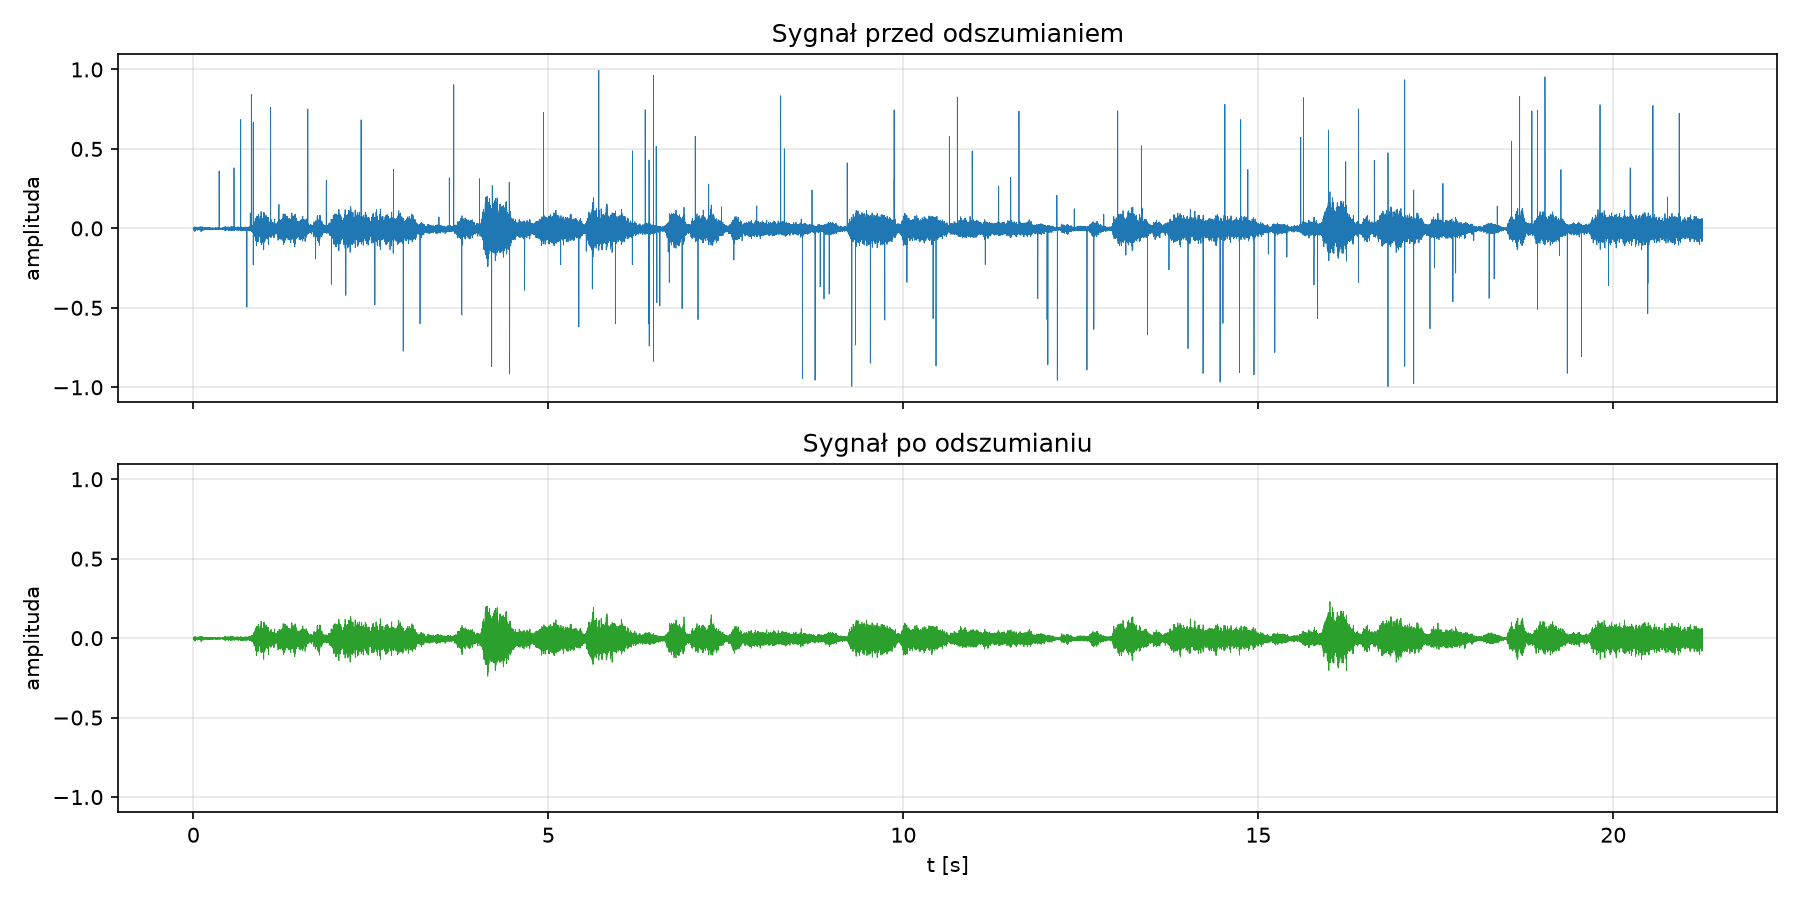
\includegraphics[width=\textwidth]{sygnal_przed_po.png}
  \caption{Sygnał przed odszumianiem (u góry) i po odszumianiu (u dołu)}
  \label{fig:sygnal}
\end{figure}

\begin{figure}[H]
  \centering
  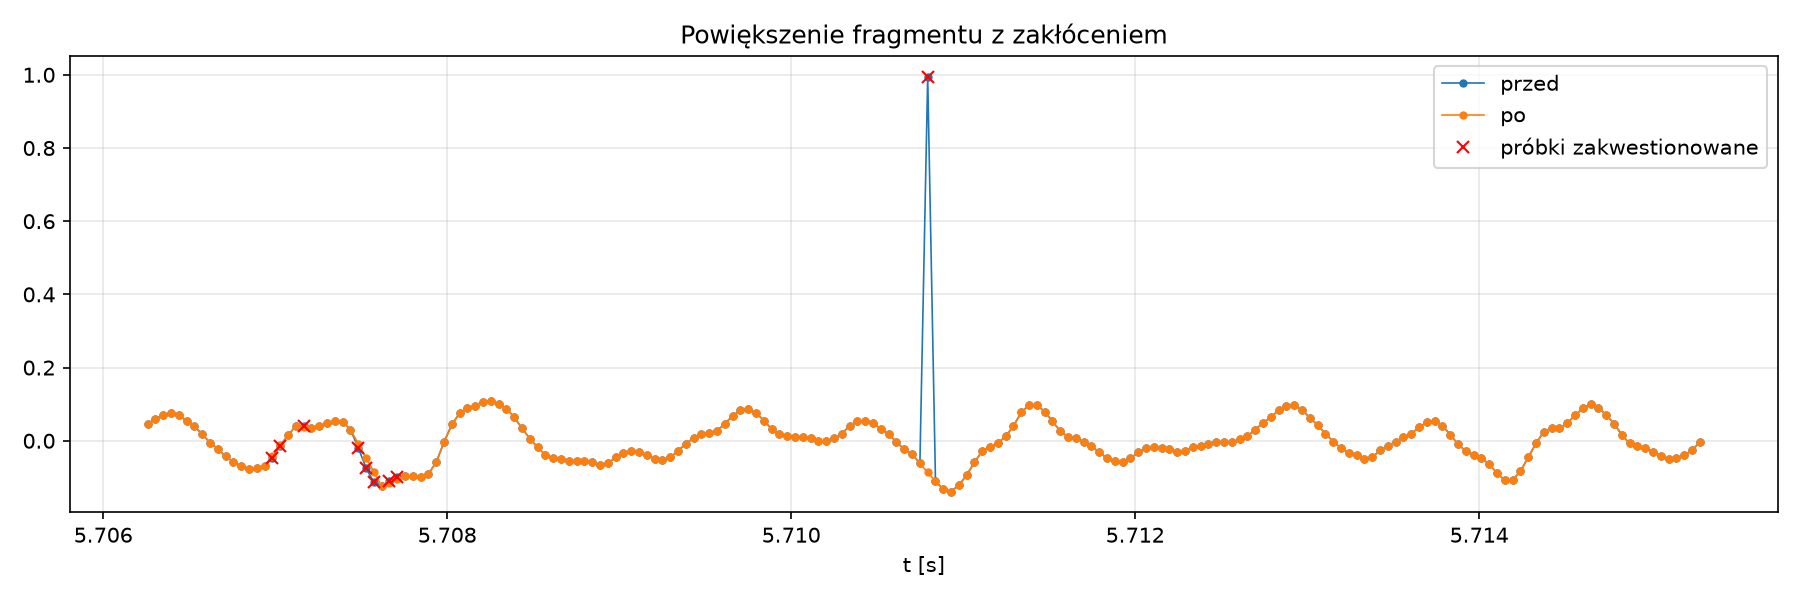
\includegraphics[width=\textwidth]{zoom.png}
  \caption{Powiększenie fragmentu z zakłóceniem o największej amplitudzie;
           krzyżykami oznaczono próbki zakwestionowane przez detektor}
  \label{fig:zoom}
\end{figure}

Przebiegi estymat parametrów modelu AR(4) pokazano na rys.~\ref{fig:ar}.
Po krótkim okresie zbieżności (około 1~s, w którym nagranie jest
prawie ciche) parametry zmieniają się w ograniczonym zakresie:
$\hat a_1 \in [0{,}5;\ 2{,}5]$, $\hat a_2 \in [-2{,}4;\ 0]$,
$\hat a_3 \in [-0{,}1;\ 1{,}3]$, $\hat a_4 \in [-0{,}55;\ 0{,}25]$.
Wyraźne skoki parametrów (np.\ przy $t\approx 2$; $4{,}5$; $6{,}6$; $8{,}8$;
$13{,}6$; $16{,}4$; $19{,}6$~s) pokrywają się ze zmianami brzmienia
nagrania: model śledzi zmiany lokalnej charakterystyki widmowej sygnału.
Trzaski nie zaburzają estymat, ponieważ próbki zakwestionowane nie są
używane do aktualizacji modelu.

\begin{figure}[H]
  \centering
  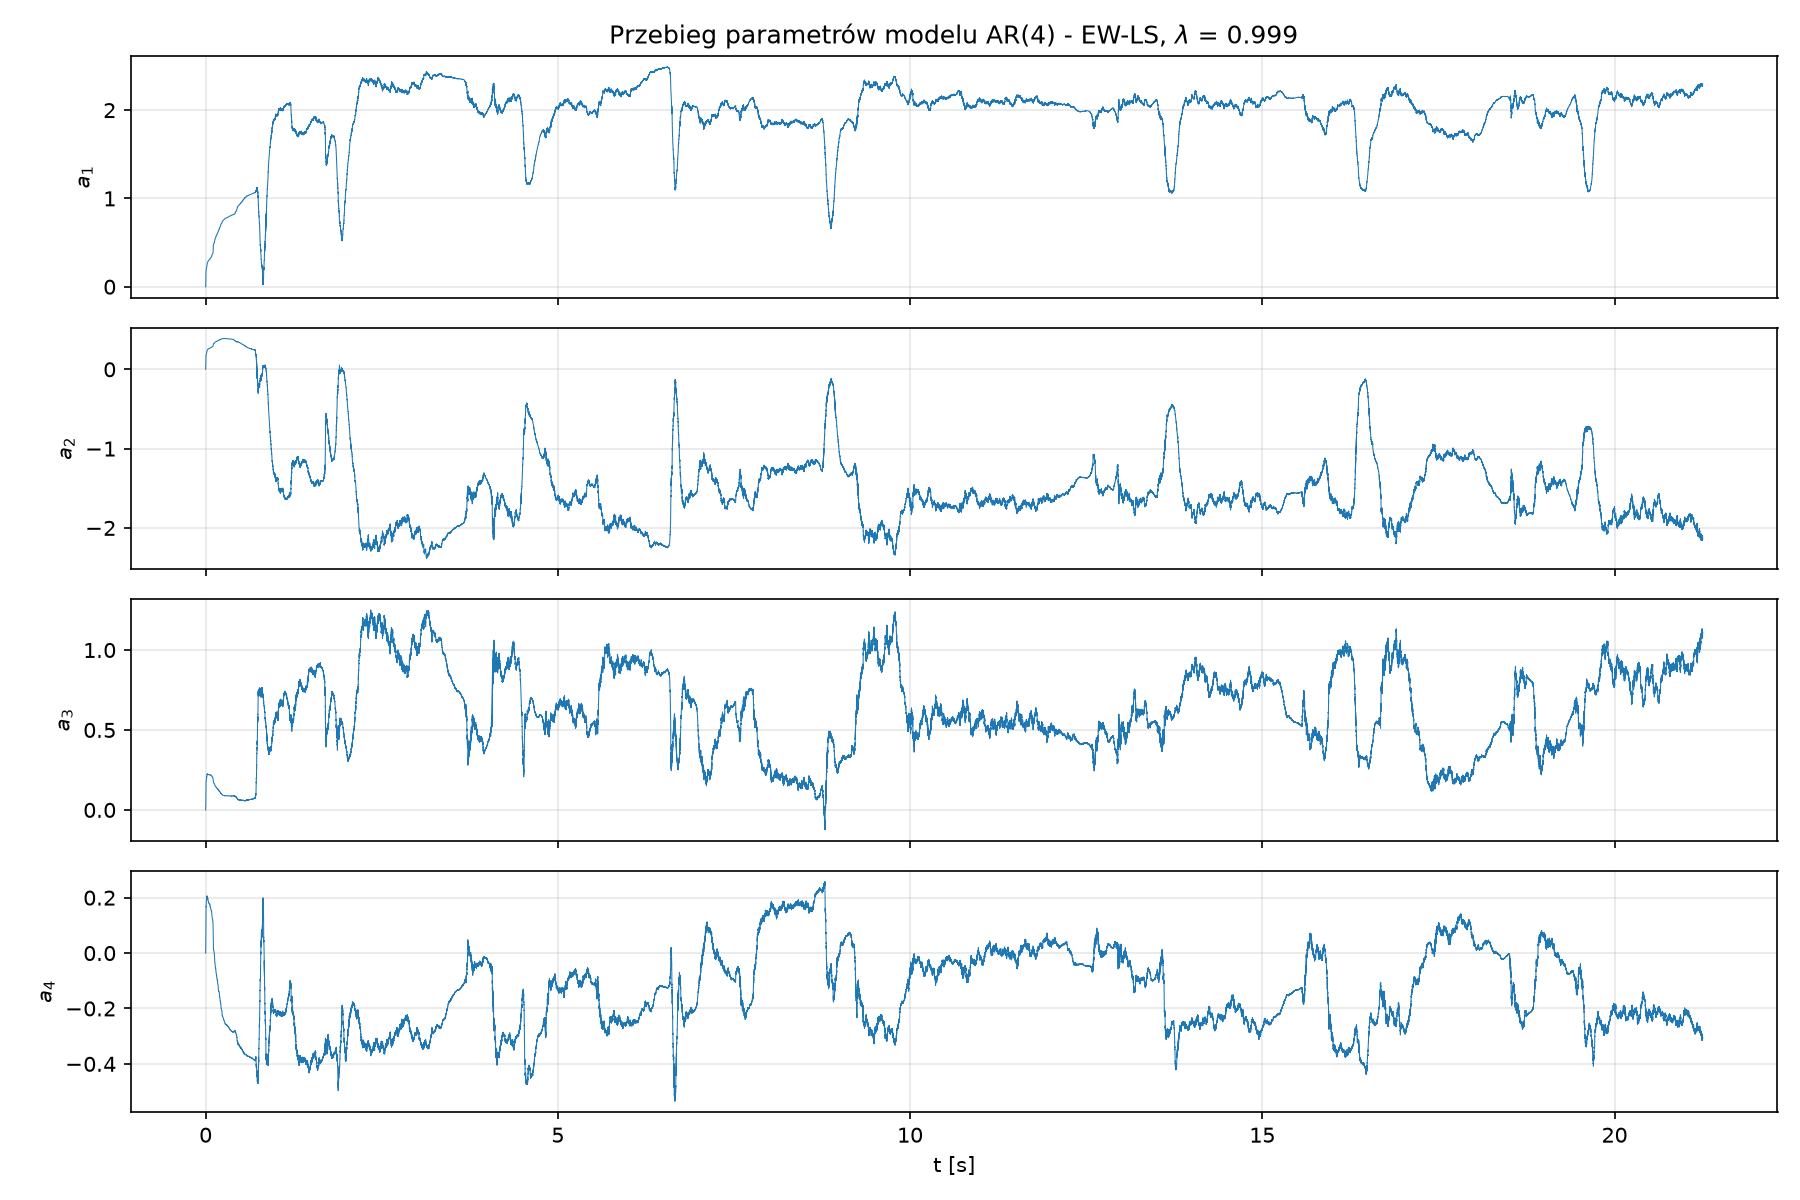
\includegraphics[width=\textwidth]{parametry_ar.png}
  \caption{Przebieg estymat parametrów $\hat a_1,\dots,\hat a_4$ modelu AR(4)}
  \label{fig:ar}
\end{figure}

Rys.~\ref{fig:prog} przedstawia moduł błędu predykcji $|\varepsilon(k)|$
na tle progu detekcji $3\hat\sigma_\varepsilon(k)$. Na górnym wykresie błędy
odpowiadające trzaskom (do około $1$) są o dwa rzędy wielkości większe niż
próg (mediana około $0{,}01$). Próg zmienia się wraz z głośnością nagrania:
we fragmentach cichych spada do około $0{,}001$, w głośnych rośnie do
$0{,}03$--$0{,}05$. Dolny wykres (powiększenie) pokazuje zachowanie detektora
w pobliżu największego trzasku.

\begin{figure}[H]
  \centering
  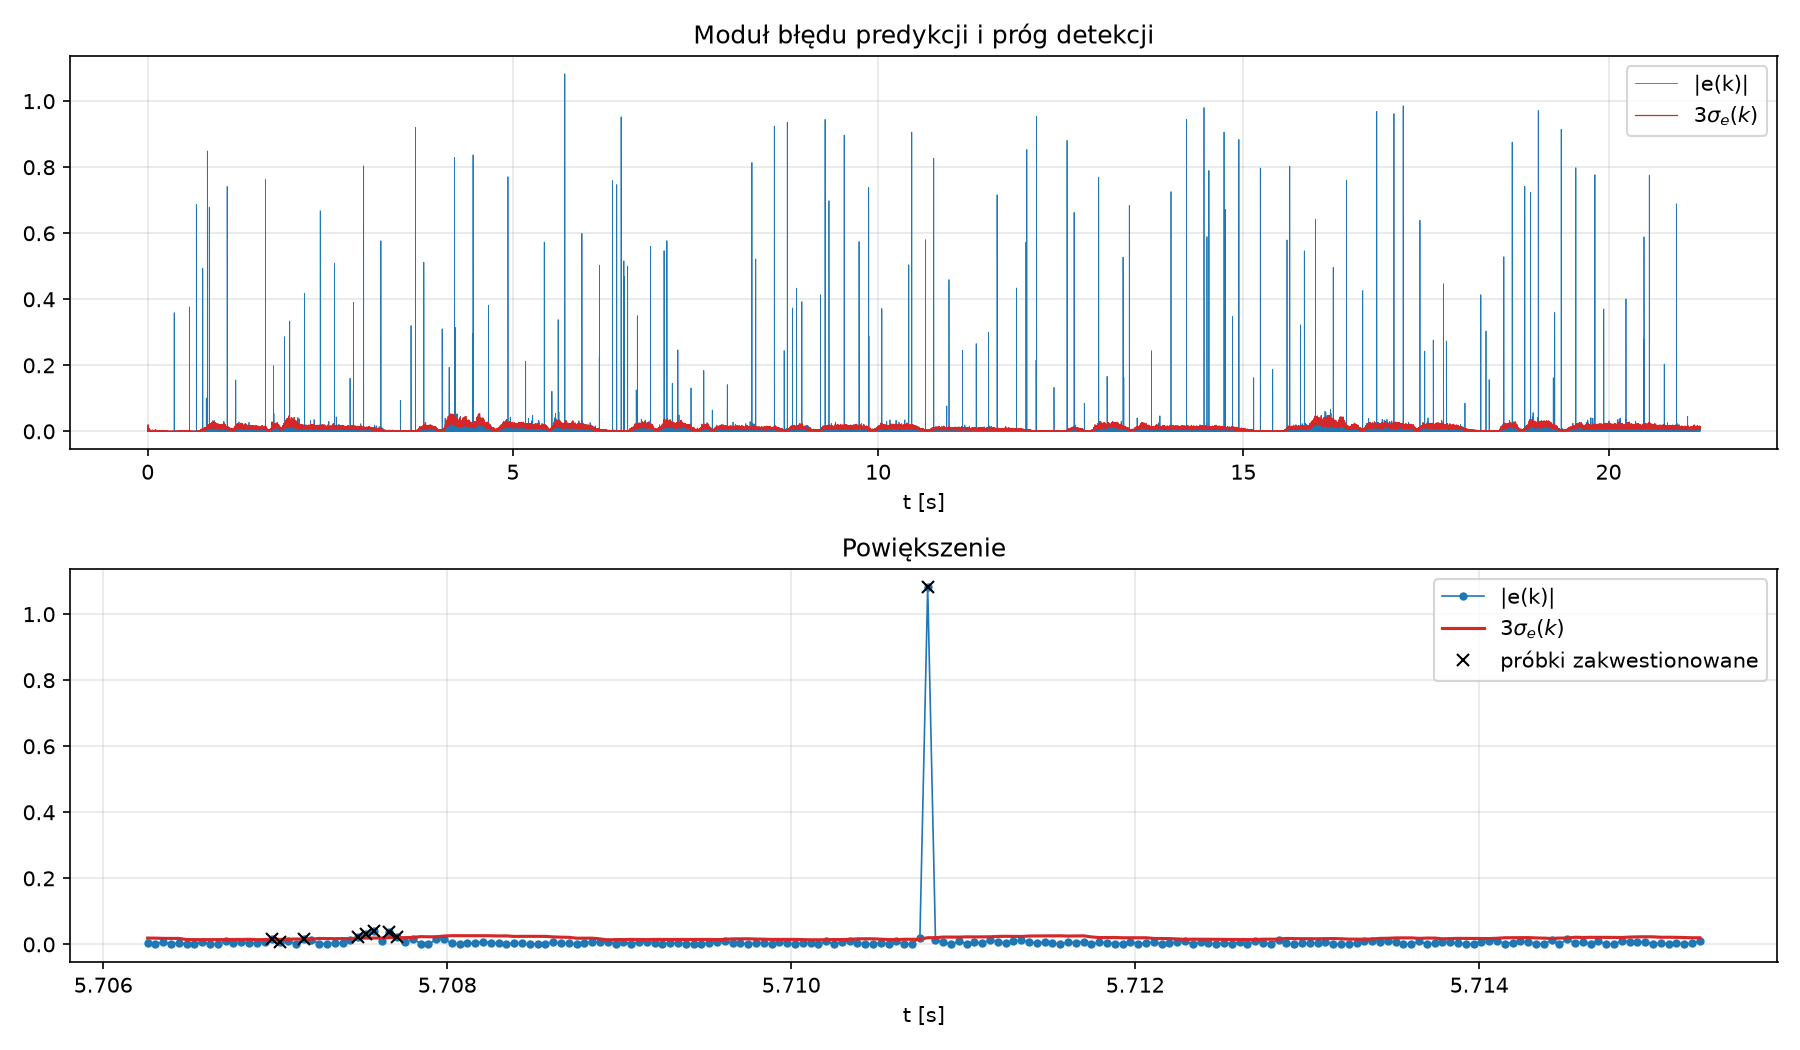
\includegraphics[width=\textwidth]{prog_detekcji.png}
  \caption{Moduł błędu predykcji i próg kwalifikujący próbkę jako błędną
           $3\hat\sigma_\varepsilon(k)$: cały sygnał (u góry) i powiększenie (u dołu)}
  \label{fig:prog}
\end{figure}

\subsection*{Ocena odsłuchowa}

Porównano odsłuchowo plik wejściowy \texttt{02.wav} z~plikiem
wynikowym \texttt{02\_odszumiony.wav}.\\ Dźwięk po odszumieniu jest bardzo czysty:
nie słychać trzasków ani szumów. Mimo dużej liczby fałszywych alarmów
detektora nie słychać też zniekształceń muzyki wynikających z interpolacji
poprawnych próbek. Potwierdza to, że zinterpolowanie pojedynczych próbek
sygnału próbkowanego z częstotliwością 22~kHz jest niesłyszalne.

%==============================================================================
\section{Wnioski}

\begin{itemize}
  \item Adaptacyjny model AR(4) identyfikowany algorytmem EW-LS wraz
        z detektorem $3\sigma$ i interpolacją liniową usunął wszystkie duże
        zakłócenia impulsowe z nagrania. Po odszumieniu nie pozostała żadna
        próbka o amplitudzie przekraczającej poziom sygnału muzycznego,
        a odsłuch potwierdza brak słyszalnych trzasków.
  \item Dla silnie skorelowanego sygnału audio algorytm EW-LS wymaga
        zabezpieczeń numerycznych: symetrycznej postaci aktualizacji
        macierzy $\mathbf{P}$ i ograniczenia jej śladu.
  \item Wektor regresji budowany z sygnału oczyszczonego (z próbkami
        zrekonstruowanymi przez interpolację) zapewnia stabilne śledzenie
        parametrów również w otoczeniu zakłóceń.
  \item Przy wyznaczaniu długości serii zakłóceń próg należy skalować
        wariancją błędu predykcji wielokrokowej; w przeciwnym razie
        w cichych fragmentach trzaski nie są wykrywane.
  \item Próg $3\sigma$ w połączeniu z krótkim oknem estymatora wariancji
        ($M = 20$, wg wykładu) daje dużą liczbę fałszywych alarmów (około
        4700 serii przy 120--200 rzeczywistych trzaskach), które jednak
        nie wpływają słyszalnie na jakość nagrania. Liczbę fałszywych
        alarmów można zmniejszyć, wydłużając okno ($M = 50$--$100$) lub
        zwiększając próg w zalecanym przedziale $\mu \in [3, 5]$.
  \item Zgodnie z treścią zadania zastosowano interpolację liniową. Lepszą
        jakość rekonstrukcji, zwłaszcza dłuższych serii, mogłaby dać
        przedstawiona w wykładzie rekonstrukcja optymalna w sensie
        średniokwadratowym, oparta na modelu AR.
\end{itemize}

%==============================================================================
\begin{thebibliography}{9}
  \bibitem{wyklad} M.~Niedźwiecki, \emph{Elimination of clicks},
    prezentacja do wykładu z przedmiotu Identyfikacja Procesów.
\end{thebibliography}

\end{document}
